\documentclass{article}\usepackage[]{graphicx}\usepackage[]{color}
%% maxwidth is the original width if it is less than linewidth
%% otherwise use linewidth (to make sure the graphics do not exceed the margin)
\makeatletter
\def\maxwidth{ %
  \ifdim\Gin@nat@width>\linewidth
    \linewidth
  \else
    \Gin@nat@width
  \fi
}
\makeatother

\definecolor{fgcolor}{rgb}{0.345, 0.345, 0.345}
\newcommand{\hlnum}[1]{\textcolor[rgb]{0.686,0.059,0.569}{#1}}%
\newcommand{\hlstr}[1]{\textcolor[rgb]{0.192,0.494,0.8}{#1}}%
\newcommand{\hlcom}[1]{\textcolor[rgb]{0.678,0.584,0.686}{\textit{#1}}}%
\newcommand{\hlopt}[1]{\textcolor[rgb]{0,0,0}{#1}}%
\newcommand{\hlstd}[1]{\textcolor[rgb]{0.345,0.345,0.345}{#1}}%
\newcommand{\hlkwa}[1]{\textcolor[rgb]{0.161,0.373,0.58}{\textbf{#1}}}%
\newcommand{\hlkwb}[1]{\textcolor[rgb]{0.69,0.353,0.396}{#1}}%
\newcommand{\hlkwc}[1]{\textcolor[rgb]{0.333,0.667,0.333}{#1}}%
\newcommand{\hlkwd}[1]{\textcolor[rgb]{0.737,0.353,0.396}{\textbf{#1}}}%

\usepackage{framed}
\makeatletter
\newenvironment{kframe}{%
 \def\at@end@of@kframe{}%
 \ifinner\ifhmode%
  \def\at@end@of@kframe{\end{minipage}}%
  \begin{minipage}{\columnwidth}%
 \fi\fi%
 \def\FrameCommand##1{\hskip\@totalleftmargin \hskip-\fboxsep
 \colorbox{shadecolor}{##1}\hskip-\fboxsep
     % There is no \\@totalrightmargin, so:
     \hskip-\linewidth \hskip-\@totalleftmargin \hskip\columnwidth}%
 \MakeFramed {\advance\hsize-\width
   \@totalleftmargin\z@ \linewidth\hsize
   \@setminipage}}%
 {\par\unskip\endMakeFramed%
 \at@end@of@kframe}
\makeatother

\definecolor{shadecolor}{rgb}{.97, .97, .97}
\definecolor{messagecolor}{rgb}{0, 0, 0}
\definecolor{warningcolor}{rgb}{1, 0, 1}
\definecolor{errorcolor}{rgb}{1, 0, 0}
\newenvironment{knitrout}{}{} % an empty environment to be redefined in TeX

\usepackage{alltt}
\usepackage{amsmath}
\usepackage{bm}

\newcommand{\trans}{^\top}
\newcommand{\link}{\ensuremath{\mathrm{link}}}
\newcommand{\mc}{\mathcal}
\newcommand{\vc}{\ensuremath{\mathrm{vec}}}
\newcommand{\code}[1]{\texttt{#1}}

\title{Random effects term for exponential decay in covariance: expDecay}
\author{Steve Walker}
\date{}
\IfFileExists{upquote.sty}{\usepackage{upquote}}{}
\begin{document}

\maketitle

One may induce covariance among the levels of a grouping factor, such
that the covariances fall off exponentially with distance among the
levels.  The distance matrix for the levels can come from many
sources, including spatial coordinates, phylogenies and other trees,
and trait space.  Such exponential decay models are specified with the
following notation.
\begin{equation}
  \label{eq:6}
  \mathtt{
    respVar \sim expDecay(1\, | \,grpFac, 
    distMat = distMat, 
    minCov = 1e-3,
    distCutoff = 2)}
\end{equation}
where \code{distMat} in an \code{R} \code{dist} object giving the
distances among levels in \code{grpFac}, and \code{minCov} and
\code{distCutoff} are parameters for trading off accuracy for
computation speed.  If \code{distCutoff > max(distMat)} and
\code{minCov == 0}, then there is no approximation but result in the
slowest speeds.  Reducing \code{distCutoff} below \code{max(distMat)}
causes all covariances associated with distances larger than
\code{distCutoff} to be zero.  Finally, \code{minCov} is the
covariance associated with \code{distCutoff}, and should be chosen to
be as low as possible.

The model has a single parameter, $\alpha$, specifying the rate of
decay.  The covariance, $\rho_{ij}$ between level $i$ and $j$ is a
function of the distance, $\delta_{ij}$, between the levels.
\begin{equation}
  \label{eq:1}
  \rho_{ij} = \exp\left(-\alpha\delta_{ij}\right)
\end{equation}

\begin{knitrout}
\definecolor{shadecolor}{rgb}{0.969, 0.969, 0.969}\color{fgcolor}
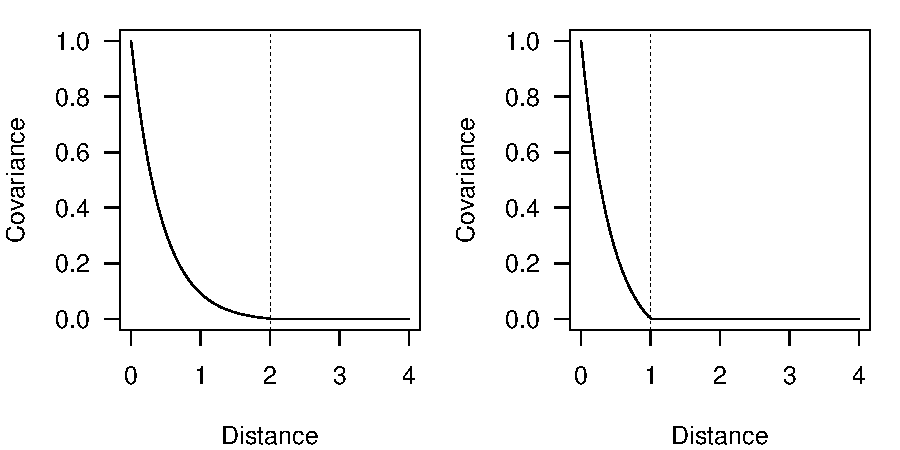
\includegraphics[width=\maxwidth]{figure/decayGraph-1} 

\end{knitrout}

\end{document}
